%\documentclass[14pt]{beamer}
\documentclass{beamer}

\usetheme{Copenhagen}
% \usetheme{Boadilla}
% \usecolortheme{beaver}
\setbeamercolor{alerted text}{fg=orange}
\setbeamercolor{background canvas}{bg=white}
\setbeamercolor{block body alerted}{bg=normal text.bg!90!black}
\setbeamercolor{block body}{bg=normal text.bg!90!black}
\setbeamercolor{block body example}{bg=normal text.bg!90!black}
\setbeamercolor{block title alerted}{use={normal text,alerted text},fg=alerted text.fg!75!normal text.fg,bg=normal text.bg!75!black}
\setbeamercolor{block title}{bg=blue}
\setbeamercolor{block title example}{use={normal text,example text},fg=example text.fg!75!normal text.fg,bg=normal text.bg!75!black}
\setbeamercolor{fine separation line}{}
\setbeamercolor{frametitle}{fg=white}
\setbeamercolor{item projected}{fg=white}
\setbeamercolor{normal text}{bg=white,fg=black}
\setbeamercolor{palette sidebar primary}{use=normal text,fg=normal text.fg}
\setbeamercolor{palette sidebar quaternary}{use=structure,fg=structure.fg}
\setbeamercolor{palette sidebar secondary}{use=structure,fg=structure.fg}
\setbeamercolor{palette sidebar tertiary}{use=normal text,fg=normal text.fg}
\setbeamercolor{section in sidebar}{fg=brown}
\setbeamercolor{section in sidebar shaded}{fg=grey}
\setbeamercolor{separation line}{}
\setbeamercolor{sidebar}{bg=red}
\setbeamercolor{sidebar}{parent=palette primary}
\setbeamercolor{structure}{bg=black, fg=white!30!blue!60!green}
\setbeamercolor{subsection in sidebar}{fg=brown}
\setbeamercolor{subsection in sidebar shaded}{fg=grey}
\setbeamercolor{title}{fg=white}
\setbeamercolor{titlelike}{fg=white}

% Szép kék
% \setbeamercolor{structure}{bg=black, fg=white!10!green!40!blue}

\frenchspacing

% Language packages
\usepackage[utf8]{inputenc}
\usepackage[T1]{fontenc}
\usepackage[magyar]{babel}

% AMS
\usepackage{amssymb,amsmath}

% Graphic packages
\usepackage{graphicx}

% Syntax highlighting
\usepackage{listings}

\usepackage{tikz}

%\begin{figure}[htb]
%\begin{center}
%	\includegraphics[scale=0.4]{ps_times.png}
%\end{center}
%\end{figure}


% ==============
\begin{document}
% ==============

\title[Strukturált adatok kinyerése PDF dokumentumokból]{Strukturált adatok kinyerése PDF dokumentumokból}
\author[Molnár Fanni]{\textbf{Molnár Fanni}}
\institute[]{Miskolci Egyetem}
\date{2020. június 23.}

% --------------------
\frame{\titlepage}

% --------------------
\begin{frame}[fragile]
\frametitle{Bevezetés}

A dokumentumaink egy jelentős része elektronikus formában érhető el. Ennek közkedvelt formátuma a PDF (Portable Document Format). 
A dolgozat olyan módszereket mutat be, amelyek a képek strukturális elemeit ismerik fel.

\smallskip

Az elemzésnek két fő alternatívája lehet:

\bigskip

\begin{itemize}
    \item PDF API-k használatával lehetn kinyerni a fájlokból a dokumentum adatait
    \item PDF képpé alakítása, majd képfeldolgozási módszerekkel való elemzése
\end{itemize}

\end{frame}

% --------------------
\begin{frame}[fragile]
\frametitle{Dokumentum szerkezete}

A dokumentumok szerkezete lehet nagyon egyszerű, de igen komplikált is.

\smallskip

\begin{figure}[!tbp]
  \centering
  \begin{minipage}[b]{0.45\textwidth}
    
\includegraphics[width=\textwidth]{images/page_simple.png}
  \end{minipage}
  \hfill
  \begin{minipage}[b]{0.45\textwidth}
    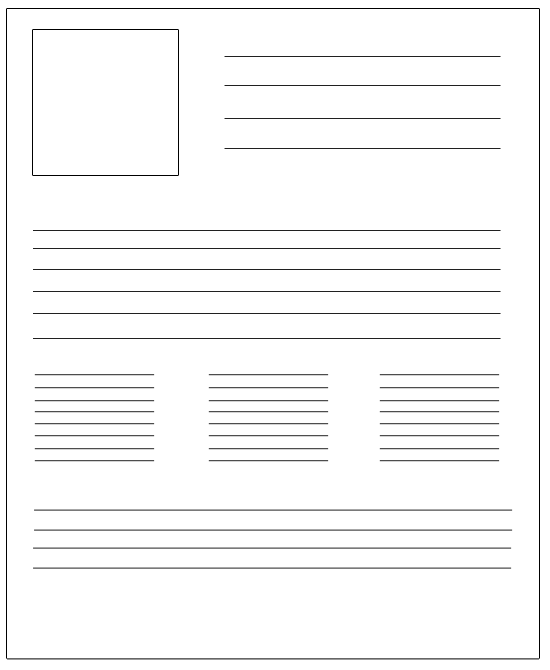
\includegraphics[width=\textwidth]{images/page_complicated}
  \end{minipage}
\end{figure}

\end{frame}

% --------------------
\begin{frame}[fragile]
\frametitle{\ }

\begin{center}

    \Large

    \textbf{Köszönöm szépen a figyelmet!}

    \bigskip

\end{center}

\end{frame}

\end{document}

